%----- Configuración del estilo del documento------%
\documentclass{report}
\usepackage[utf8]{inputenc}

%----- Paquete para algunos fonts ------%
\usepackage[T1]{fontenc}

%----- Paquete para configurar los márgenes del documento ------%
\usepackage[left=2.5cm,right=2.5cm,top=1.8cm,bottom=2.3cm]{geometry}

%----- Paquete para imagenes ------%
\usepackage{graphicx}

% ----- Paquete para matemáticas ------%
\usepackage{amsmath,amssymb,amsthm}

%----- Paquete para encabezados,pies de pagina y tabla de contenidos ------%
\usepackage{fancyhdr,lastpage,tocloft}

%----- Estilo personalizado para mi tabla de contenido ------%  
\renewcommand{\cfttoctitlefont}{\LARGE\bfseries}
\renewcommand{\cftchapfont}{\large\bfseries}
\renewcommand{\cftsecfont}{\normalsize\itshape}
\setlength{\cftbeforechapskip}{1em}
\setlength{\cftbeforesecskip}{0.5em}
\renewcommand{\cftchapleader}{\cftdotfill{\cftdotsep}}

%----- Paquete para tablas ------%
\usepackage[shortlabels]{enumitem}

%----- Paquete para hipervinculos ------%
\usepackage{hyperref}

%------ Paquetes para color ------------%
\usepackage{xcolor}

% ------ Paquetes para la bibliografía ------%
\usepackage[backend=biber]{biblatex}
\addbibresource{resources/referencias/referencias.bib}
\usepackage{csquotes}


\begin{document}
    \begin{titlepage}
	\thispagestyle{empty}
	\begin{minipage}[c][0.17\textheight][c]{0.21\textwidth}
		\begin{center}
			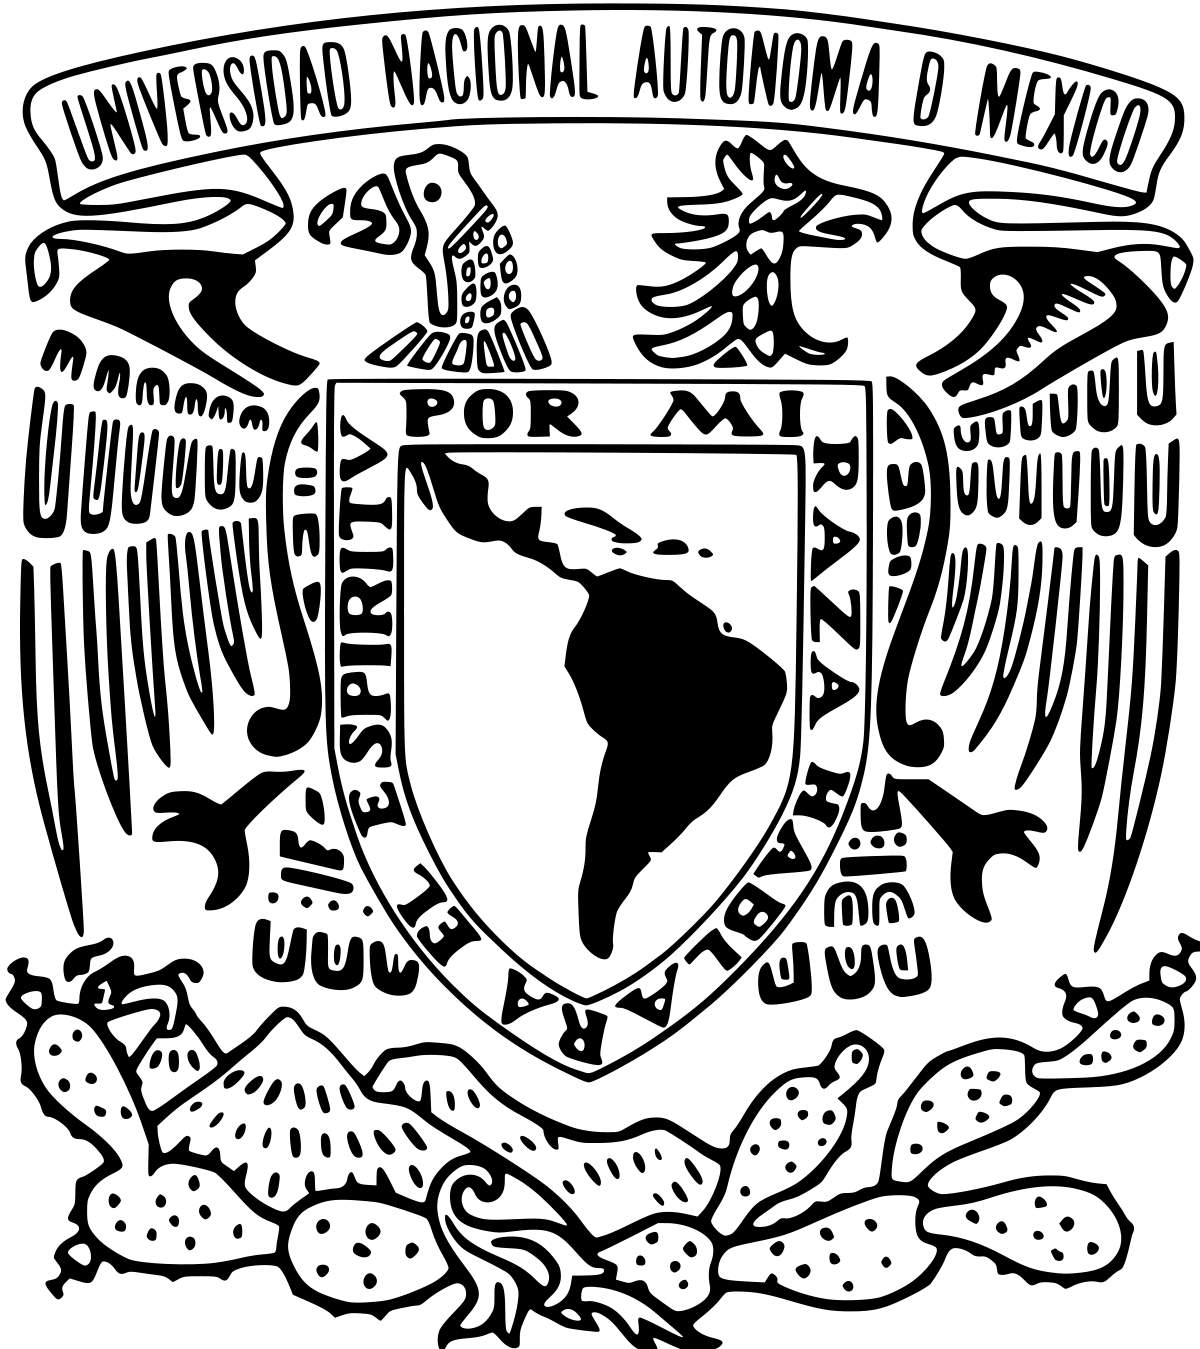
\includegraphics[width=3.2cm, height=3.5cm]{resources/Logo_UNAM.png}
		\end{center}
	\end{minipage}
	\begin{minipage}[c][0.195\textheight][t]{0.75\textwidth}
		\begin{center}
			\vspace{0.3cm}
			\textsc{\large Universidad Nacional Aut\'onoma de M\'exico}\\[0.5cm]
			\vspace{0.3cm}		
			\hrule height2.5pt
			\vspace{.2cm}
			\hrule height1pt
			\vspace{.8cm}
			\textsc{Facultad de Ciencias}\\[0.5cm] %
		\end{center}
	\end{minipage}
	
	\begin{minipage}[c][0.81\textheight][t]{0.21\textwidth}
		\vspace*{5mm}
		\begin{center}
			\hskip2.0mm
			\vrule width1pt height13cm 
			\vspace{5mm}
			\hskip2pt
			\vrule width2.5pt height13cm
			\hskip2mm
			\vrule width1pt height13cm \\
			\vspace{5mm}
			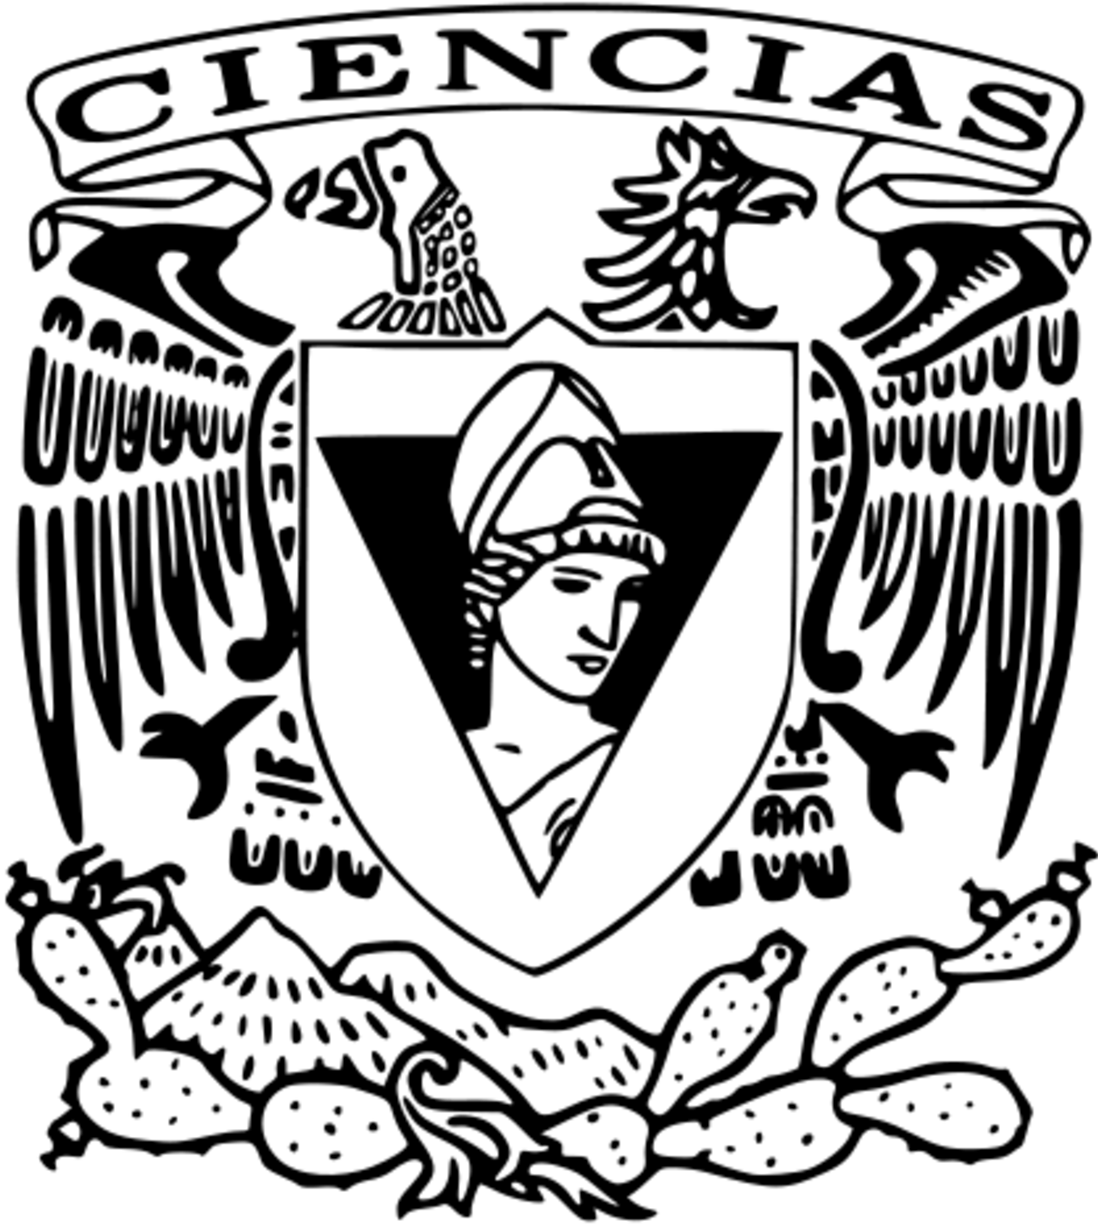
\includegraphics[height=4.0cm, width=3.2cm]{resources/Logo_FC.png}
		\end{center}
	\end{minipage}
	\begin{minipage}[c][0.81\textheight][t]{0.75\textwidth}
		\begin{center}
			\vspace{1cm}
			
			{\large\scshape Computación Distribuida - 7176}\\[.2in]
			
			\vspace{2cm}            
			
			\textsc{\LARGE \textbf{P}\hspace{1cm}\textbf{R}\hspace{1cm}\textbf{O}\hspace{1cm}\textbf{Y}\hspace{1cm}\textbf{E}\hspace{1cm}\textbf{C}\hspace{1cm}\textbf{T}\hspace{1cm}\textbf{O}}\\[2cm]

			\textsc{\Large{Equipo:}\normalsize \\
                \vspace{.3cm}
				\textbf{Ángeles Sánchez Aldo Javier - 320286144 \\
				\vspace{.2cm}
				Sánchez Victoria Leslie Paola - 320170513 \\
				\vspace{.2cm}
				\href{https://github.com/JuanSosaCiencias}{\textcolor{blue}{Sosa Romo Juan Mario - 320051926}} }}\\[0.5cm]     
			
			\textsc{{Fecha de entrega: \\ \textbf{29 de Noviembre de 2024}}}\\[0.5cm]        
			
			\textsc{{Profesor: \\ \textbf{Mat. Salvador López Mendoza}}}\\[0.5cm]  
			
			\textsc{Ayudante: \\ \textbf{Santiago Arroyo Lozano } }
			
			
			\vspace{0.5cm}
		\end{center}
	\end{minipage}
\end{titlepage}
 % Portada del documento

    % Índice
    \tableofcontents

    % Explicar el problema
    \chapter{\LARGE{Planteamiento del problema}}
    \vspace{-.6cm}
{\large {
    Este documento presenta la solución final al proyecto de la materia de Computación Distribuida. El objetivo de este trabajo es desarrollar una blockchain para un sistema de criptomonedas, implementado en el lenguaje de programación \textit{Elixir}. \vspace{.6cm}

    Durante la ejecución del proyecto, se simulará el sistema de criptomonedas gestionando los distintos procesos distribuidos que representan a los usuarios. Estos usuarios realizarán transacciones entre ellos, enviando mensajes para alcanzar un consenso y detectando y eliminando intentos de alteración de la cadena de bloques. La blockchain, aunque simula un entorno, debe operar de forma descentralizada y garantizar la integridad de la información, asegurando que los nodos honestos mantengan una copia consistente de las transacciones para que estas se validen e inserten correctamente. \vspace{.6cm}

    Para modelar las conexiones de la red, se utiliza una implementación basada en el modelo \textit{Watts y Strogatz}, que garantiza un coeficiente de agrupamiento alto y una estructura que favorece la propagación eficiente de la información. Se asegura que este coeficiente sea mayor a 0.4 para comenzar el proceso de consenso y transmisión de transacciones. \vspace{.6cm}

    Una de las características importantes del proyecto es la introducción de \textbf{procesos} \textbf{bizantinos}, los cuales representan nodos maliciosos en la red. Estos procesos se encargan de generar bloques basura o incorrectos con la intención de alterar la blockchain y comprometer su integridad. Sin embargo, el sistema debe ser capaz de detectar y evitar que estos bloques maliciosos sean insertados en la cadena. Para garantizar la seguridad y la correcta operación de la red, se asume que, si hay $f$ nodos bizantinos y $n$ nodos en total, se cumple la condición $ n > 3f $, lo que asegura que la mayoría de los nodos honestos puedan mantener la coherencia de la blockchain. \vspace{.6cm}

    \textbf{Consideraciones extra}  \vspace{.6cm}

    Se pueden utilizar cuantas funciones auxiliares sean necesarias, siempre que se logre el objetivo deseado. No es necesario implementar la persistencia del estado o la validación de la cartera; una vez que el programa termina, la blockchain deja de existir, y no se almacenará nada de forma permanente. No se realizará ninguna verificación sobre la validez de las transacciones en cuanto a saldo disponible. Se proporcionará un módulo inicial llamado \textit{Crypto} encargado de realizar los hasheos de los bloques. Finalmente, la red debe ser capaz de evitar la inserción de bloques generados por procesos bizantinos, manteniendo así la integridad del sistema.
}}


    % Explicar la solución propuesta
    \chapter{\LARGE{Solución propuesta}}

    \section{\Large{Flujo general de la solución}}
    
\vspace{1cm}
{\Huge{\textbf{Primer Idea}}} 
\vspace{1cm}

{\large{

    Proceso de Inserción de un Bloque en la Blockchain  \vspace{.3cm}

    Supongamos que inicialmente la Blockchain solo está compuesta por al menos el bloque *“Genesis Block”* y que existe un nodo A que desea insertar un bloque a la Blockchain.  \vspace{.3cm}

    Si el nodo A crea un bloque, este debe ser válido por sí solo, es decir, al menos debe contar con la siguiente información:

    \begin{itemize}
        \item \texttt{data}: La información de transacción.
        \item \texttt{timestamp}: Fecha y hora de la creación del bloque.
        \item \texttt{prev\_hash}: Último hash de la Blockchain.
        \item \texttt{hash}: Hash del bloque actual.  \vspace{.3cm}
    \end{itemize}

    \textbf{Nota}: La creación de este bloque implica el uso del módulo \texttt{Crypto}.  \vspace{.3cm}

    Si el bloque no cumple con los requisitos mínimos, este es desechado automáticamente.  \vspace{.3cm}

    Si el bloque es válido, este se difunde al resto de nodos en la red.  \vspace{.3cm}

    Para cada nodo que ha recibido el bloque nuevo, se debe validar que este tiene el hash correcto del bloque anterior con respecto a la versión de la Blockchain que dispone cada uno. Además, se debe verificar que la fecha del nuevo bloque sea mayor que la del bloque previo a este.  \vspace{.3cm}

    Si el bloque es válido, este se añade a la Blockchain. En otro caso, se desecha.  \vspace{.3cm}

    Después de la inserción, se verifica cuál es la Blockchain correcta (la más larga) para compartir esta versión a los nodos que se quieran unir a la red.  \vspace{.3cm}

    Para ello, sea \textit{bc} una estructura auxiliar que guardará la Blockchain que, por el momento, tiene la mayoría y sea \textit{mayoría} una variable auxiliar que cuenta cuántos nodos tienen la misma Blockchain que \textit{bc}.  \vspace{.3cm}

    Inicialmente, se toma un nodo de la red y se supone que su Blockchain es la correcta; se copia su información a \textit{bc} y se establece \textit{mayoría = 0}. Tomamos el siguiente nodo para revisar su versión de la Blockchain comparándolo con \textit{bc}.  \vspace{.3cm}

    \begin{itemize}
        \item Si las dos Blockchains son iguales, se incrementa en uno \textit{mayoría}.
        \item Si son diferentes, se toma como la verdadera Blockchain la que se está revisando y se actualiza \textit{bc}.  \vspace{.3cm}
    \end{itemize}

    Para las siguientes rondas, si \textit{mayoría} > 0 y la Blockchain que se está revisando es distinta a \textit{bc}, disminuimos en uno \textit{mayoría}. Cuando \textit{mayoría} sea igual a cero, actualizamos \textit{bc}.  \vspace{.3cm}

    El algoritmo termina cuando se hayan revisado todas las Blockchains.
}}

\vspace{1cm}
{\Huge{\textbf{Segunda Idea}}} 
\vspace{1cm}

{\large{
    \textbf{1. Inicialización del Sistema:}
    \begin{itemize}
        \item \textbf{Entrada:} El programa recibe dos parámetros principales:
        \begin{itemize}
            \item $n$: Número de nodos en la red.
            \item $f$: Número de nodos bizantinos.
        \end{itemize}
        \item \textbf{Configuración de la Red:}
        \begin{itemize}
            \item \textit{Modelo Watts y Strogatz:} Se configura la topología de la red con base en este modelo, asegurando que el coeficiente de agrupamiento sea mayor a 0.4 antes de comenzar el proceso. Este modelo garantiza que los nodos estén interconectados de manera eficiente para propagar la información.
            \item \textbf{Creación de Nodos:} Se crean $n$ nodos, de los cuales $f$ son bizantinos, generando un total de $n - f$ nodos honestos, asegurando la desigualdad $n > 3f$ para mantener la integridad de la red.
        \end{itemize}
    \end{itemize}

    \vspace{0.5cm}

    \textbf{2. Creación de Procesos y Asignación de Roles:}
    \begin{itemize}
        \item \textbf{Spawning de Procesos:} Los nodos se representan como procesos concurrentes en Elixir, cada uno responsable de gestionar la lógica de su respectivo nodo en la blockchain.
        \item \textbf{Asignación de Roles:}
        \begin{itemize}
            \item \textbf{Nodos honestos:} Serán responsables de validar y propagar transacciones y bloques correctos.
            \item \textbf{Nodos bizantinos:} Estos nodos generarán bloques maliciosos o basura, intentado alterar la blockchain y perturbar el consenso.
        \end{itemize}
    \end{itemize}

    \vspace{0.5cm}

    \textbf{3. Generación de Bloques:}
    \begin{itemize}
        \item \textbf{Proceso de Bloques:}
        \begin{itemize}
            \item Cada nodo (honesto o bizantino) genera bloques de acuerdo con los datos que quiere insertar en la blockchain.
            \item Un bloque incluye:
            \begin{itemize}
                \item \texttt{data}: El contenido de la transacción o mensaje.
                \item \texttt{timestamp}: La hora en la que se generó el bloque.
                \item \texttt{prev\_hash}: El hash del bloque anterior.
                \item \texttt{hash}: El hash del bloque actual generado a partir de los datos.
            \end{itemize}
        \end{itemize}
        \item \textbf{Validación de Bloques:}
        \begin{itemize}
            \item Los nodos validan los bloques según la regla de que cada bloque debe contener un hash válido del bloque anterior.
            \item Los bloques generados por los nodos bizantinos se detectan como inválidos y no se insertan en la blockchain.
        \end{itemize}
    \end{itemize}

    \vspace{0.5cm}

    \textbf{4. Proceso de Consenso:}
    \begin{itemize}
        \item \textbf{Comunicación entre Nodos:}
        \begin{itemize}
            \item Los nodos honestos intercambian información entre sí para llegar a un consenso sobre la validez de los bloques.
            \item Se utiliza un protocolo de consenso \textbf{CAMBIAR ESTO} donde los nodos honestos verifican si los bloques propuestos cumplen con las reglas del sistema.
        \end{itemize}
        \item \textbf{Bloques Maliciosos:}
        \begin{itemize}
            \item Los nodos bizantinos intentan insertar bloques maliciosos en la blockchain. Sin embargo, debido a la validación y el consenso de la red, estos bloques no se aceptan, y se descartan.
        \end{itemize}
    \end{itemize}

    \vspace{0.5cm}

    \textbf{5. Validación de la Blockchain:}
    \begin{itemize}
        \item \textbf{Validación Continua:}
        \begin{itemize}
            \item En todo momento, la blockchain debe validarse para asegurarse de que no haya bloques comprometidos. Esta validación se realiza mediante la comparación de los bloques, verificando que el hash de un bloque coincida con el \texttt{prev\_hash} del siguiente bloque.
        \end{itemize}
        \item \textbf{Redefinición de la Blockchain:}
        \begin{itemize}
            \item Si se detecta una alteración significativa o corrupción en la blockchain (debido a bloques maliciosos de nodos bizantinos), la blockchain puede ser descartada y se puede iniciar una nueva cadena.
        \end{itemize}
    \end{itemize}

    \vspace{0.5cm}

    \textbf{6. Inserción de Nuevos Bloques:}
    \begin{itemize}
        \item \textbf{Proceso de Inserción:}
        \begin{itemize}
            \item Cuando un bloque es validado correctamente, se inserta en la blockchain.
            \item La cadena se mantiene actualizada y es replicada en los nodos honestos.
        \end{itemize}
    \end{itemize}

    \vspace{0.5cm}

    \textbf{7. Finalización:}
    \begin{itemize}
        \item \textbf{Detención del Programa:}
        \begin{itemize}
            \item Una vez que el proceso de simulación ha terminado, el programa termina, y la blockchain se elimina de la memoria. No se realiza persistencia de datos.
            \item Se puede consultar el estado final de la blockchain en la terminal para verificar que las transacciones se han propagado correctamente y que los bloques maliciosos fueron descartados.
        \end{itemize}
    \end{itemize}

    \vspace{0.5cm}

    \textbf{Resumen Visual del Flujo:}
    \begin{enumerate}
        \item \textbf{Inicialización:} Parámetros ($n$, $f$) → Topología de Red (Modelo Watts y Strogatz) → Creación de Nodos (honestos y bizantinos)
        \item \textbf{Generación de Bloques:} Nodos crean bloques (datos, timestamp, prev\_hash, hash)
        \item \textbf{Validación de Bloques:} Nodos validan bloques, descartan bloques maliciosos de nodos bizantinos.
        \item \textbf{Proceso de Consenso:} Nodos honestos alcanzan consenso, bloques correctos son insertados.
        \item \textbf{Validación Continua de la Blockchain:} Se valida la cadena para asegurar que no haya corrupción de datos.
        \item \textbf{Inserción de Nuevos Bloques:} Bloques válidos son insertados y replicados entre nodos honestos.
        \item \textbf{Finalización:} Programa termina, blockchain se elimina (sin persistencia).
    \end{enumerate}
}}

    % \section{\Large{Consenso}}
    % \large{
Para el consenso, el equipo decidió utilizar el algoritmo ya creado, \textbf{pBFT}; para la información de esta sección se utilizaron las referencias: \cite{geeksforgeeks_pbft} \cite{castro_liskov_1999}. 

La primera es más accesible y proporciona las bases del algoritmo, mientras que la segunda es más técnica, siendo el paper original. Este segundo recurso es útil para profundizar en el tema. 

Antes de explicar el consenso, los problemas que el algoritmo busca resolver son:
\begin{itemize}
    \item \textbf{Nodos Bizantinos:} Habrá nodos maliciosos que envíen mensajes incorrectos a la red. Nuestro sistema debe tolerarlos y alcanzar un consenso a pesar de su presencia.
    \item \textbf{Errores en los mensajes:} En una red real, los mensajes pueden perderse, retrasarse o llegar desordenados; asumimos que siempre llegan eventualmente. El sistema debe tolerar estos problemas y alcanzar el consenso.
    \item \textbf{Consistencia:} Todos los nodos honestos deben consensuar el orden de los bloques y validar su legitimidad.
    \item \textbf{Validez:} El consenso alcanzado no debe incluir bloques corruptos generados por nodos maliciosos.
\end{itemize}

}

\section*{El Algoritmo pBFT}

El algoritmo \textbf{pBFT} sigue tres etapas principales para llegar al consenso:

\begin{enumerate}
    \item \textbf{Preparación Inicial (Pre-Prepare):} 
    Un nodo propone un mensaje para ser aceptado por la red. Este mensaje, llamado \textit{preprepare}, contiene un identificador único (hash o timestamp) y el bloque propuesto.

    \item \textbf{Preparación (Prepare):} 
    Los nodos que reciben un mensaje \textit{preprepare} validan el bloque. Si es válido, envían un mensaje \textit{prepare} a sus vecinos. Cada nodo acumula mensajes \textit{prepare}. Si recibe al menos \(2f + 1\) mensajes válidos (incluido el suyo), pasa a la siguiente etapa.

    \item \textbf{Compromiso (Commit):} 
    En esta fase, el nodo envía un mensaje \textit{commit} a todos sus vecinos. Si un nodo acumula \(2f + 1\) mensajes \textit{commit} válidos, acepta el bloque y lo agrega a su \texttt{blockchain} local.
\end{enumerate}

Aunque el algoritmo tiene una complejidad de comunicación \(O(n^2)\), consideramos que esto es manejable para redes pequeñas o medianas.


    \section{\Large{Módulos y sus funciones}}
    \large{
\section*{Archivo \textbf{Blockchain.ex}:}
\section*{Módulo \texttt{Block}}

\subsection*{\texttt{new/2}}
\begin{verbatim}
new(data, prev_hash)
\end{verbatim}

Crea un nuevo bloque con los datos proporcionados (\texttt{data}) y el hash del bloque previo (\texttt{prev\_hash}).

\[
\text{timestamp} = \text{DateTime.utc\_now()} \rightarrow \text{Fecha y hora actuales en formato UTC.}
\]

Se genera un bloque inicial con un hash vacío y luego se calcula el hash del bloque usando el módulo \texttt{Crypto}:

\[
\text{block.hash} = \text{Crypto.put\_hash(block)}
\]

\subsection*{\texttt{valid?/1}}
\begin{verbatim}
valid?(%Block{})
\end{verbatim}

Valida que un bloque sea correcto verificando si el hash almacenado coincide con el hash calculado a partir de los datos del bloque.

\[
\text{valid} = \text{block.hash} == \text{Crypto.hash(block)}
\]

\subsection*{\texttt{valid?/2}}
\begin{verbatim}
valid?(%Block{}, %Block{})
\end{verbatim}

Valida que dos bloques consecutivos sean correctos. Comprueba lo siguiente:

\begin{itemize}
    \item El \texttt{prev\_hash} del segundo bloque coincide con el \texttt{hash} del primer bloque.
    \item El orden temporal entre los bloques es correcto: \texttt{block1.timestamp} $\leq$ \texttt{block2.timestamp}.
    \item Ambos bloques son válidos individualmente: \texttt{Block.valid?(block1)} y \texttt{Block.valid?(block2)}.
\end{itemize}

\section*{Módulo \texttt{Blockchain}}

\subsection*{\texttt{new\_genesis\_block/0}}
\begin{verbatim}
new_genesis_block()
\end{verbatim}

Crea el bloque génesis, que es el primer bloque de la blockchain. Este bloque contiene:

\begin{itemize}
    \item \texttt{data}: "Genesis Block".
    \item \texttt{timestamp}: "2024-01-01 00:00:00Z".
    \item \texttt{prev\_hash}: "0".
\end{itemize}

El hash se calcula con \texttt{Crypto.put\_hash(block)}.

\subsection*{\texttt{new/0}}
\begin{verbatim}
new()
\end{verbatim}

Inicializa una nueva blockchain con el bloque génesis. Retorna una estructura de tipo \texttt{Blockchain}:

\[
\text{blockchain} = \%Blockchain\{\text{chain}: [\text{genesis\_block}]\}
\]

\subsection*{\texttt{valid?/1}}
\begin{verbatim}
valid?(%Blockchain{})
\end{verbatim}

Valida toda la blockchain asegurándose de que:

\begin{itemize}
    \item El hash de cada bloque coincide con el calculado para ese bloque.
    \item El \texttt{prev\_hash} de cada bloque coincide con el \texttt{hash} del bloque anterior.
    \item Los bloques están ordenados cronológicamente.
\end{itemize}

Utiliza \texttt{Enum.chunk\_every(2, 1, :discard)} para generar pares consecutivos de bloques, y luego verifica la validez de cada par con \texttt{Block.valid?/2}.

\subsection*{\texttt{insert/2}}
\begin{verbatim}
insert(%Block{}, %Blockchain{})
\end{verbatim}

Inserta un nuevo bloque en la blockchain. Verifica que:

\begin{itemize}
    \item Existe un bloque previo (\texttt{List.last(chain)}).
    \item El nuevo bloque es válido en relación con el último bloque: \texttt{Block.valid?(last\_block, new\_block)}.
\end{itemize}

Si todo está en orden, entonces el nuevo bloque se añade a la cadena:

\[
\text{updated\_chain} = \text{chain} ++ [\text{new\_block}]
\]

Si no está en orden, retorna un error indicando que el bloque no es válido.\\

%%%%%%%%%%%%%%%%%%%%%%%%%%%%%%%%%

\section*{Archivo \textbf{Grafica.ex}:}

\section*{Módulo \texttt{Grafica}}

\subsection*{\texttt{inicia/1}}
\begin{verbatim}
inicia(estado_inicial \\ %{})
\end{verbatim}

Inicializa un nodo con un estado inicial, que incluye:

\begin{itemize}
    \item \texttt{vecinos}: lista de otros nodos con los que se comunica.
    \item \texttt{blockchain}: blockchain actual del nodo (inicializada con \texttt{Blockchain.new()}).
    \item \texttt{bizantino}: indica si el nodo es malicioso (\texttt{true}) o no (\texttt{false}).
    \item \texttt{mensajes}: estructura para almacenar mensajes de tipo \texttt{prepare} y \texttt{commit}.
\end{itemize}

El nodo llama a \texttt{recibe\_mensaje/1} para comenzar a procesar mensajes.

\subsection*{\texttt{recibe\_mensaje/1}}
\begin{verbatim}
recibe_mensaje(estado)
\end{verbatim}

Espera y procesa mensajes recibidos de otros nodos. Llama a \texttt{procesa\_mensaje/2} para manejar cada mensaje y actualiza el estado del nodo.

\subsection*{\texttt{procesa\_mensaje/2}}
\begin{verbatim}
procesa_mensaje(mensaje, estado)
\end{verbatim}

Procesa diferentes tipos de mensajes. Los cuales son:

\paragraph{\texttt{Estado}}
Muestra el estado actual del nodo y reinicia los mensajes.

\[
\text{estado} = \text{reiniciar\_mensajes\_y\_vistos(estado)}
\]

\paragraph{\texttt{Vecinos}}
Asigna una lista de vecinos al nodo y actualiza su estado.

\[
\text{estado} = \text{Map.put(estado, :vecinos, vecinos)}
\]

\paragraph{\texttt{Bloque}}
Envía un bloque a los vecinos. Si el nodo es bizantino, envía un bloque modificado con datos corruptos.

\paragraph{\texttt{Preprepare}}
Procesa un mensaje \texttt{preprepare}. Si el bloque es válido, envía un mensaje \texttt{prepare} a los vecinos.

\paragraph{\texttt{Prepare}}
Procesa un mensaje \texttt{prepare}. Si el nodo no ha visto el mensaje antes, lo agrega a sus mensajes y verifica si se alcanza un cuórum. Si el cuórum es suficiente, envía un mensaje \texttt{commit}.

\paragraph{\texttt{Commit}}
Procesa un mensaje \texttt{commit}. Si el nodo no ha visto el mensaje antes, lo agrega a la blockchain una vez alcanzado el cuórum.

\subsection*{\texttt{reiniciar\_mensajes\_y\_vistos/1}}
\begin{verbatim}
reiniciar_mensajes_y_vistos(estado)
\end{verbatim}

Reinicia los mensajes (\texttt{prepare} y \texttt{commit}) y limpia la lista de mensajes vistos.

\[
\text{estado} = \text{Map.put(estado, :mensajes, \%{:prepare => [], :commit => []})}
\]

\subsection*{\texttt{actualizar\_mensajes/3}}
\begin{verbatim}
actualizar_mensajes(estado, tipo, mensaje)
\end{verbatim}

Agrega un mensaje a la lista correspondiente (\texttt{prepare} o \texttt{commit}).

\[
\text{mensajes\_actualizados} = \text{Map.update(estado[:mensajes], tipo, [mensaje], {[mensaje | \&1]})}
\]

\subsection*{\texttt{suficiente\_cuorum?/2}}
\begin{verbatim}
suficiente_cuorum?(estado, tipo)
\end{verbatim}

Verifica si se alcanzó un cuórum para un tipo de mensaje (\texttt{prepare} o \texttt{commit}). Calcula un umbral basado en la cantidad de nodos:

\[
\text{threshold} = \left\lfloor \frac{2 \cdot (\text{total\_nodos})}{3} \right\rfloor + 1
\]

Retorna \texttt{true} si el número de mensajes únicos es suficiente para alcanzar el cuórum.

\subsection*{\texttt{agregar\_bloque/2}}
\begin{verbatim}
agregar_bloque(bloque, estado)
\end{verbatim}

Agrega un bloque a la blockchain del nodo si es válido. Si ocurre un error, mantiene el estado actual.

\subsection*{\texttt{mensaje\_visto?/2}}
\begin{verbatim}
mensaje_visto?(estado, mensaje)
\end{verbatim}

Verifica si un mensaje ya ha sido visto por el nodo. Utiliza un conjunto (\texttt{MapSet}) para comprobar duplicados.

\subsection*{\texttt{marcar\_mensaje\_visto/2}}
\begin{verbatim}
marcar_mensaje_visto(estado, mensaje)
\end{verbatim}

Marca un mensaje como visto y lo añade al conjunto \texttt{mensajes\_vistos}.

%%%%%%%%%%%%%%%%%%%%%%
\section*{Archivo \textbf{Crypto.ex}:}
\section*{Módulo \texttt{Crypto}}

El módulo \texttt{Crypto} asegura la integridad de los bloques en una blockchain.

\subsection*{Atributo de Módulo}
\begin{verbatim}
@block_fields [:data, :timestamp, :prev_hash]
\end{verbatim}

Define los campos del bloque (\texttt{data}, \texttt{timestamp} y \texttt{prev\_hash}) que serán utilizados para calcular su hash.

\subsection*{\texttt{hash/1}}
\begin{verbatim}
hash(%{} = block)
\end{verbatim}

Calcula el hash criptográfico de un bloque.

\paragraph{Parámetros}
\begin{itemize}
    \item \texttt{block}: Un mapa que representa un bloque, utilizando \texttt{@block\_fields}.
\end{itemize}

\paragraph{Retorno}
\begin{itemize}
    \item Una cadena que representa el hash calculado para el bloque.
\end{itemize}


\subsection*{\texttt{put\_hash/1}}
\begin{verbatim}
put_hash(%{} = block)
\end{verbatim}

Calcula e inserta el hash en un bloque.

\paragraph{Parámetros}
\begin{itemize}
    \item \texttt{block}: Un mapa que representa un bloque.
\end{itemize}

\paragraph{Retorno}
\begin{itemize}
    \item El bloque actualizado con un nuevo campo \texttt{:hash}, que contiene el hash calculado.
\end{itemize}

\paragraph{Funcionamiento}
\begin{enumerate}
    \item Llama a la función \texttt{hash/1} para calcular el hash del bloque.
    \item Devuelve el bloque con el campo \texttt{:hash} actualizado.
\end{enumerate}

\subsection*{\texttt{encode\_to\_binary/1}}
\begin{verbatim}
encode_to_binary(map)
\end{verbatim}

Convierte un mapa en una representación binaria.

\paragraph{Parámetros}
\begin{itemize}
    \item \texttt{map}: Un mapa cuyos valores serán convertidos a binario.
\end{itemize}

\paragraph{Retorno}
\begin{itemize}
    \item Una lista de caracteres binarios que representan el mapa.
\end{itemize}

\paragraph{Funcionamiento}
\begin{enumerate}
    \item Convierte cada valor del mapa a binario mediante la función \texttt{to\_binary/1}.
    \item Une los valores binarios en una cadena.
    \item Convierte la cadena a una lista binaria con \texttt{:erlang.binary\_to\_list/1}.
\end{enumerate}

\subsection*{\texttt{to\_binary/1}}
\begin{verbatim}
to_binary(value)
\end{verbatim}

Convierte un valor individual en su representación binaria.

\paragraph{Parámetros}
\begin{itemize}
    \item \texttt{value}: Un valor de cualquier tipo.
\end{itemize}

\paragraph{Retorno}
\begin{itemize}
    \item Una representación binaria del valor. Si ya es binario, se retorna tal cual; de lo contrario, se convierte usando \texttt{inspect/1}.
\end{itemize}

\subsection*{\texttt{simple\_hash/1}}
\begin{verbatim}
simple_hash(binary)
\end{verbatim}

Calcula un hash sencillo a partir de una cadena binaria.

\paragraph{Parámetros}
\begin{itemize}
    \item \texttt{binary}: Una cadena binaria de entrada.
\end{itemize}

\paragraph{Retorno}
\begin{itemize}
    \item Una cadena hexadecimal que representa el hash calculado.
\end{itemize}

\paragraph{Funcionamiento}
\begin{enumerate}
    \item Utiliza la función \texttt{:erlang.phash2/1} para calcular el hash de la cadena.
    \item Convierte el valor resultante a una cadena hexadecimal con \texttt{Integer.to\_string/2}.
\end{enumerate}

%%%%%%%%%%%%%%%%%%%%%%%%%%%%%%%%

\section*{Archivo Main.ex}

\section*{Módulo \texttt{Main}}
Este módulo controla la creación de una red de nodos utilizando el modelo de Watts y Strogatz. Simula una blockchain distribuida donde los nodos se comunican y llegan a consenso mediante el algoritmo PBFT.

\subsection*{\texttt{run/2}}
\begin{verbatim}
run(n, f)
\end{verbatim}

Inicializa una red de nodos, simula el consenso enviando bloques válidos e inválidos y verifica los estados finales.

\paragraph{Parámetros:}
\begin{itemize}
    \item \texttt{n}: Número total de nodos en la red.
    \item \texttt{f}: Número de nodos bizantinos en la red.
\end{itemize}

\paragraph{Retorno:}
\begin{itemize}
    \item Lista de procesos de nodos creados.
\end{itemize}

\paragraph{Funcionamiento:}
\begin{enumerate}
    \item Crea nodos (honestos y bizantinos) mediante \texttt{crea\_nodos/2}.
    \item Asigna vecinos a los nodos utilizando el modelo de Watts y Strogatz en \texttt{asigna\_vecinos/1}.
    \item Simula el envío y la propagación de bloques válidos e inválidos.
    \item Verifica el estado final de los nodos.
\end{enumerate}

\subsection*{\texttt{crea\_nodos/2}}
\begin{verbatim}
crea_nodos(n, f)
\end{verbatim}

Crea una lista de nodos que incluye:
\begin{itemize}
    \item \texttt{f} nodos bizantinos creados con \texttt{NodoBizantino.inicia/0}.
    \item \texttt{n-f} nodos honestos creados con \texttt{NodoHonesto.inicia/0}.
\end{itemize}

\paragraph{Retorno:}
\begin{itemize}
    \item Lista de procesos de nodos creados.
\end{itemize}

\subsection*{\texttt{asigna\_vecinos/1}}
\begin{verbatim}
asigna_vecinos(procesos)
\end{verbatim}

Asigna vecinos a los nodos de la red, utilizando un modelo en anillo con probabilidades de reconexión aleatoria.

\paragraph{Funcionamiento:}
\begin{enumerate}
    \item Asigna a cada nodo \texttt{k} vecinos iniciales en un anillo.
    \item Introduce conexiones aleatorias con probabilidad de reenlace \texttt{0.1}.
    \item Verifica que el coeficiente de agrupamiento sea mayor a \texttt{0.4}.
\end{enumerate}

\paragraph{Retorno:}
Ninguno. Envía mensajes con los vecinos asignados a cada nodo.

\subsection*{\texttt{clustering\_coefficient/2}}
\begin{verbatim}
clustering_coefficient(vecinos, procesos)
\end{verbatim}

Calcula el coeficiente de agrupamiento de la red.

\paragraph{Parámetros:}
\begin{itemize}
    \item \texttt{vecinos}: Lista de listas que representa los vecinos de cada nodo.
    \item \texttt{procesos}: Lista de procesos de los nodos.
\end{itemize}

\paragraph{Retorno:}
\begin{itemize}
    \item El coeficiente de agrupamiento (promedio del número de triángulos formados por los nodos).
\end{itemize}

---

\section*{Módulo \texttt{NodoHonesto}}
Simula un nodo honesto que participa de manera no maliciosa en la red.

\subsection*{\texttt{inicia/0}}
\begin{verbatim}
inicia()
\end{verbatim}

Inicia un nodo honesto con un estado inicial:

\begin{itemize}
    \item \texttt{vecinos}: Lista de vecinos asignados.
    \item \texttt{blockchain}: Blockchain inicializada.
    \item \texttt{bizantino}: \texttt{false}.
    \item \texttt{mensajes}: Diccionario vacío para almacenar mensajes \texttt{prepare} y \texttt{commit}.
\end{itemize}

Llama a \texttt{Grafica.inicia/1} para iniciar el nodo.

---

\section*{Módulo \texttt{NodoBizantino}}
Simula un nodo bizantino que actúa de manera maliciosa en la red.

\subsection*{\texttt{inicia/0}}
\begin{verbatim}
inicia()
\end{verbatim}

Inicia un nodo bizantino con un estado inicial:

\begin{itemize}
    \item \texttt{vecinos}: Lista de vecinos asignados.
    \item \texttt{blockchain}: Blockchain inicializada.
    \item \texttt{bizantino}: \texttt{true}.
    \item \texttt{mensajes}: Diccionario vacío para almacenar mensajes \texttt{prepare} y \texttt{commit}.
\end{itemize}

Llama a \texttt{Grafica.inicia/1} para iniciar el nodo.

}



    
    % Resultados
    \chapter{\LARGE{Resultados}}

    \section{\Large{Implementación}}
    \input{resources/Chapters/Resultados/resultados.tex}

    \section{\Large{Pruebas}}
    \input{resources/Chapters/Resultados/pruebas.tex}

    \section{\Large{Notas de los resultados}}
    \input{resources/Chapters/Resultados/notas.tex}

    % Conclusiones
    \chapter{\LARGE{Conclusiones}}
    \large{
Durante la implementación de nuestra variante del algoritmo \texttt{Practical Byzantine Fault Tolerance (PBFT)}, llegamos a las siguientes conclusiones:\\

- \textbf{Eliminación del líder:}\\ 
   Permitimos que cualquier nodo propusiera bloques, eliminando la dependencia del líder. Esto simplificó la lógica aunque incrementó el volumen de mensajes.\\

- \textbf{Topología de red:} \\
   Usar el modelo de \texttt{Watts y Strogatz} permitió una rápida propagación de mensajes gracias a un alto coeficiente de agrupamiento. \\

- \textbf{Tolerancia a nodos bizantinos:}\\
   Suponiendo que hay \(f\) nodos bizantinos, el algoritmo funciona correctamente en configuraciones de \(3f + 1\), logrando consenso a pesar de las fallas. \\

En conclusión, implementamos una solución descentralizada basada en \texttt{PBFT} adaptada a redes distribuidas. Es posible escalar el proyecto y asegurarse que funcione correctamente en más escenarios, como varios procesos intentando mandar mensaje al mismo tiempo. 
}


    % Bibliografía
    \newpage  
    \chapter*{Referencias}
    \addcontentsline{toc}{chapter}{Referencias}
    \printbibliography
\end{document}
